% Diagrama de flujo de la validación de frecuencias mediante FFT (nodo 1).
% Compilar: pdflatex diagrama_flujo_validacion.tex
\documentclass[tikz,border=6pt]{standalone}
\usepackage[utf8]{inputenc}
\usepackage[T1]{fontenc}
\usepackage{helvet}
\renewcommand{\familydefault}{\sfdefault}
\usepackage{courier}
\usepackage{amsmath}
\usetikzlibrary{positioning,arrows.meta,shapes.geometric,shapes.misc,calc}

\begin{document}
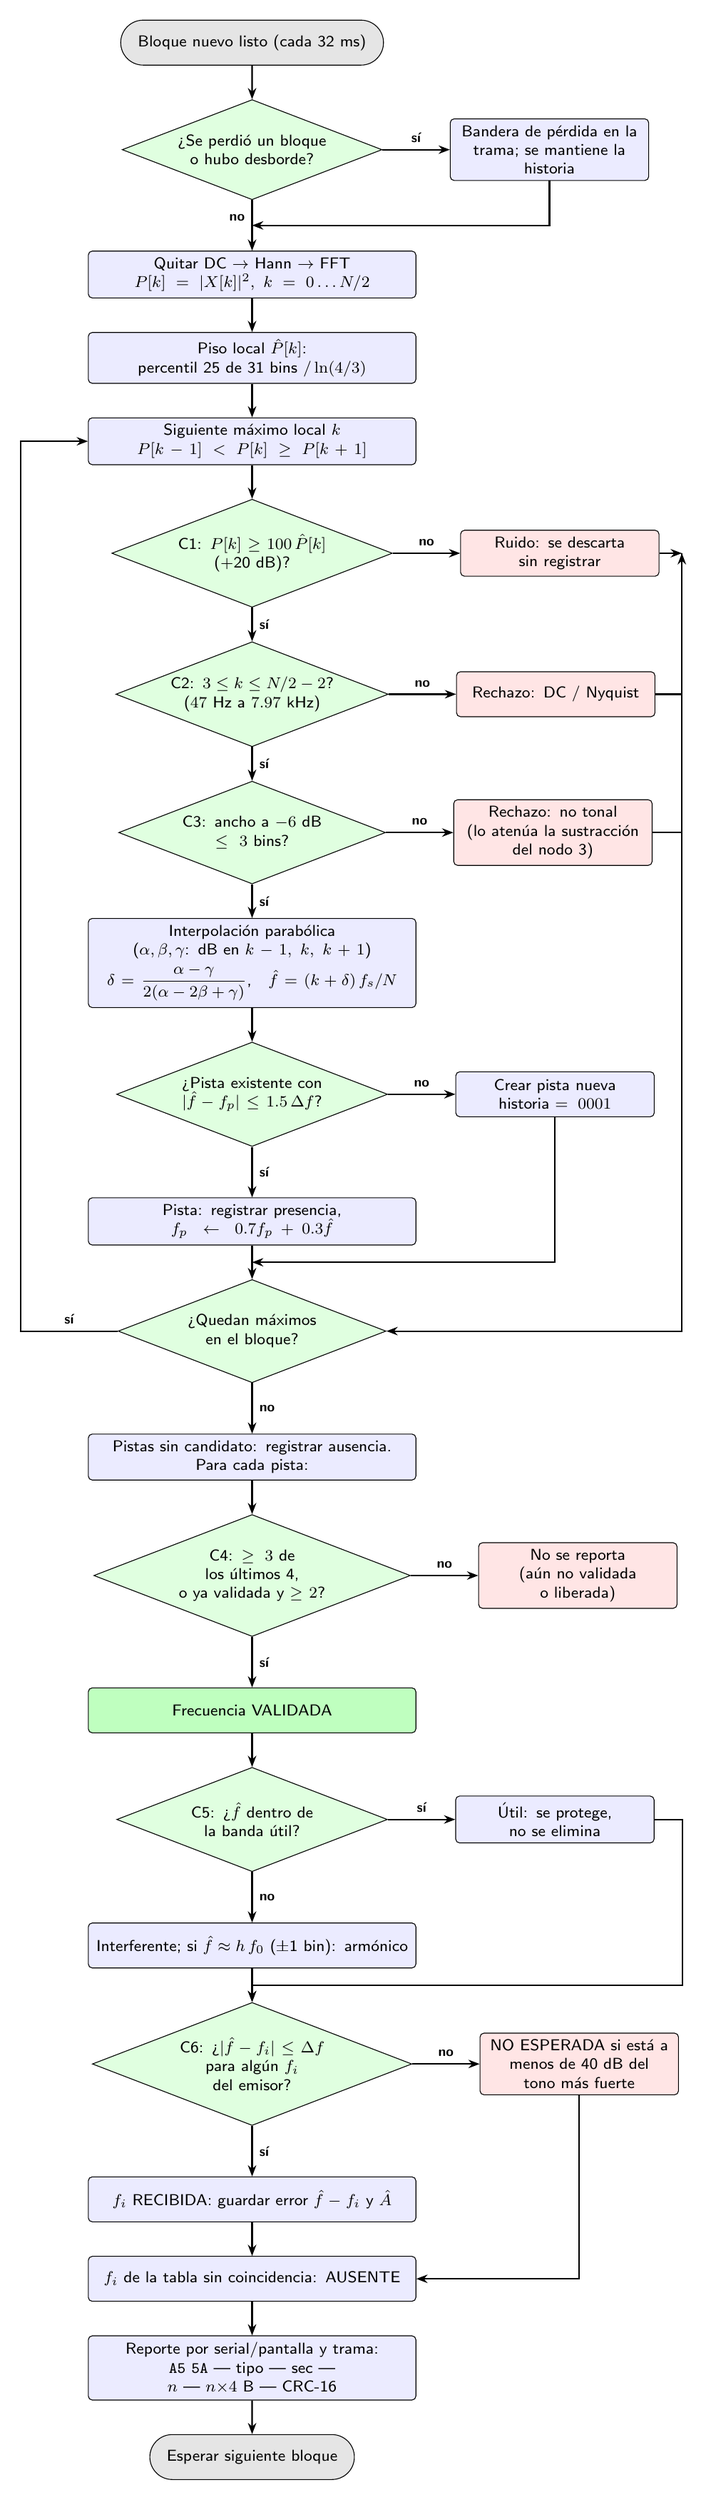
\begin{tikzpicture}[
  font=\footnotesize,
  node distance=6mm,
  >={Stealth[length=2mm]},
  inicio/.style={draw, rounded rectangle, fill=gray!20, align=center, minimum height=8mm,
                 inner xsep=8pt},
  proc/.style={draw, rounded corners=2pt, fill=blue!8, align=center, text width=56mm,
               minimum height=8mm},
  dec/.style={draw, diamond, aspect=2.6, fill=green!12, align=center, inner sep=1pt,
              text width=30mm},
  fin/.style={draw, rounded corners=2pt, fill=red!10, align=center, text width=33mm,
              minimum height=8mm},
  ok/.style={draw, rounded corners=2pt, fill=green!25, align=center, text width=56mm,
             minimum height=8mm},
  linea/.style={->, thick},
  et/.style={font=\scriptsize\bfseries}
]

\node[inicio] (ini) {Bloque nuevo listo (cada 32 ms)};
\node[dec, below=of ini] (ovf) {¿Se perdió un bloque\\o hubo desborde?};
\node[proc, below=9mm of ovf] (fft) {Quitar DC $\rightarrow$ Hann $\rightarrow$ FFT\\
  $P[k]=|X[k]|^2,\ k=0\ldots N/2$};
\node[proc, below=of fft] (piso) {Piso local $\hat P[k]$:\\percentil 25 de 31 bins $/\ln(4/3)$};
\node[proc, below=of piso] (max) {Siguiente máximo local $k$\\$P[k-1] < P[k] \ge P[k+1]$};
\node[dec, below=of max] (c1) {C1: $P[k] \ge 100\,\hat P[k]$\\(+20 dB)?};
\node[dec, below=of c1] (c2) {C2: $3 \le k \le N/2-2$?\\($47$ Hz a $7.97$ kHz)};
\node[dec, below=of c2] (c3) {C3: ancho a $-6$ dB\\$\le 3$ bins?};
\node[proc, below=of c3] (int) {Interpolación parabólica\\($\alpha,\beta,\gamma$: dB en $k-1,\ k,\ k+1$)\\[2pt]
  $\delta=\dfrac{\alpha-\gamma}{2(\alpha-2\beta+\gamma)}$,\quad $\hat f=(k+\delta)\,f_s/N$};
\node[dec, below=of int] (match) {¿Pista existente con\\$|\hat f - f_p| \le 1.5\,\Delta f$?};
\node[proc, below=9mm of match] (upd) {Pista: registrar presencia,\\$f_p \leftarrow 0.7 f_p + 0.3 \hat f$};
\node[dec, below=of upd] (mas) {¿Quedan máximos\\en el bloque?};
\node[proc, below=9mm of mas] (aus) {Pistas sin candidato: registrar ausencia.\\Para cada pista:};
\node[dec, below=of aus] (c4) {C4: $\ge 3$ de los últimos 4,\\o ya validada y $\ge 2$?};
\node[ok, below=9mm of c4] (val) {Frecuencia VALIDADA};
\node[dec, below=of val] (c5) {C5: ¿$\hat f$ dentro de\\la banda útil?};
\node[proc, below=9mm of c5] (int2) {Interferente; si $\hat f \approx h\,f_0$ (±1 bin): armónico};
\node[dec, below=of int2] (c6) {C6: ¿$|\hat f - f_i| \le \Delta f$\\para algún $f_i$ del emisor?};
\node[proc, below=9mm of c6] (rec) {$f_i$ RECIBIDA: guardar error $\hat f - f_i$ y $\hat A$};
\node[proc, below=of rec] (aus2) {$f_i$ de la tabla sin coincidencia: AUSENTE};
\node[proc, below=of aus2] (tx) {Reporte por serial/pantalla y trama:\\
  \texttt{A5 5A} | tipo | sec | $n$ | $n{\times}4$ B | CRC-16};
\node[inicio, below=of tx] (end) {Esperar siguiente bloque};

% Rechazos (columna derecha)
\node[fin, right=12mm of c1] (r1) {Ruido: se descarta\\sin registrar};
\node[fin, right=12mm of c2] (r2) {Rechazo: DC / Nyquist};
\node[fin, right=12mm of c3] (r3) {Rechazo: no tonal\\(lo atenúa la sustracción\\del nodo 3)};
\node[proc, text width=33mm, right=12mm of match] (nueva) {Crear pista nueva\\historia $= 0001$};
\node[fin, right=12mm of c4] (lib) {No se reporta\\(aún no validada\\o liberada)};
\node[proc, text width=33mm, right=12mm of c5] (util) {Útil: se protege,\\no se elimina};
\node[proc, text width=33mm, right=12mm of ovf] (flag) {Bandera de pérdida en la\\trama; se mantiene la\\historia};

% Flujo principal
\draw[linea] (ini) -- (ovf);
\draw[linea] (ovf) -- node[et, left, pos=0.35] {no} (fft);
\draw[linea] (ovf) -- node[et, above] {sí} (flag);
\draw[linea] (flag.south) |- ($(fft.north)!0.5!(ovf.south)$);
\draw[linea] (fft) -- (piso);
\draw[linea] (piso) -- (max);
\draw[linea] (max) -- (c1);
\draw[linea] (c1) -- node[et, right] {sí} (c2);
\draw[linea] (c2) -- node[et, right] {sí} (c3);
\draw[linea] (c3) -- node[et, right] {sí} (int);
\draw[linea] (int) -- (match);
\draw[linea] (match) -- node[et, right] {sí} (upd);
\draw[linea] (upd) -- (mas);
\draw[linea] (mas) -- node[et, right] {no} (aus);
\draw[linea] (aus) -- (c4);
\draw[linea] (c4) -- node[et, right] {sí} (val);
\draw[linea] (val) -- (c5);
\draw[linea] (c5) -- node[et, right] {no} (int2);
\draw[linea] (int2) -- (c6);
\draw[linea] (c6) -- node[et, right] {sí} (rec);
\draw[linea] (rec) -- (aus2);
\draw[linea] (aus2) -- (tx);
\node[fin, right=12mm of c6] (noesp) {NO ESPERADA si está a\\menos de 40 dB del\\tono más fuerte};
\draw[linea] (c6) -- node[et, above] {no} (noesp);
\draw[linea] (noesp.south) |- (aus2.east);
\draw[linea] (tx) -- (end);

% Ramas laterales
\draw[linea] (c1) -- node[et, above] {no} (r1);
\draw[linea] (c2) -- node[et, above] {no} (r2);
\draw[linea] (c3) -- node[et, above] {no} (r3);
\draw[linea] (match) -- node[et, above] {no} (nueva);
\draw[linea] (nueva.south) |- ($(upd.south)!0.5!(mas.north)$);
\draw[linea] (c4) -- node[et, above] {no} (lib);
\draw[linea] (c5) -- node[et, above] {sí} (util);
\draw[linea] (util.east) -- ++(5mm,0) |- ($(c6.north)+(0,3mm)$) -- (c6.north);

% Lazo: volver por el siguiente máximo (por la izquierda)
\coordinate (izq) at ($(max.west)+(-12mm,0)$);
\draw[linea] (mas.west) -- node[et, above] {sí} (mas.west -| izq) -- (izq) -- (max.west);
\draw[linea] (r1.east) -- ++(4mm,0) coordinate (der);
\draw[linea] (r2.east) -| (der);
\draw[linea] (r3.east) -| (der) |- ($(mas.east)+(0,0)$);

\end{tikzpicture}
\end{document}
